\chapter{SQL Injections and CAPTCHAs}

\section{SQL injections}
Structured query language (SQL) is the language used to interact with and manage data stored in a database.

\begin{figure}[H]
  \centering
  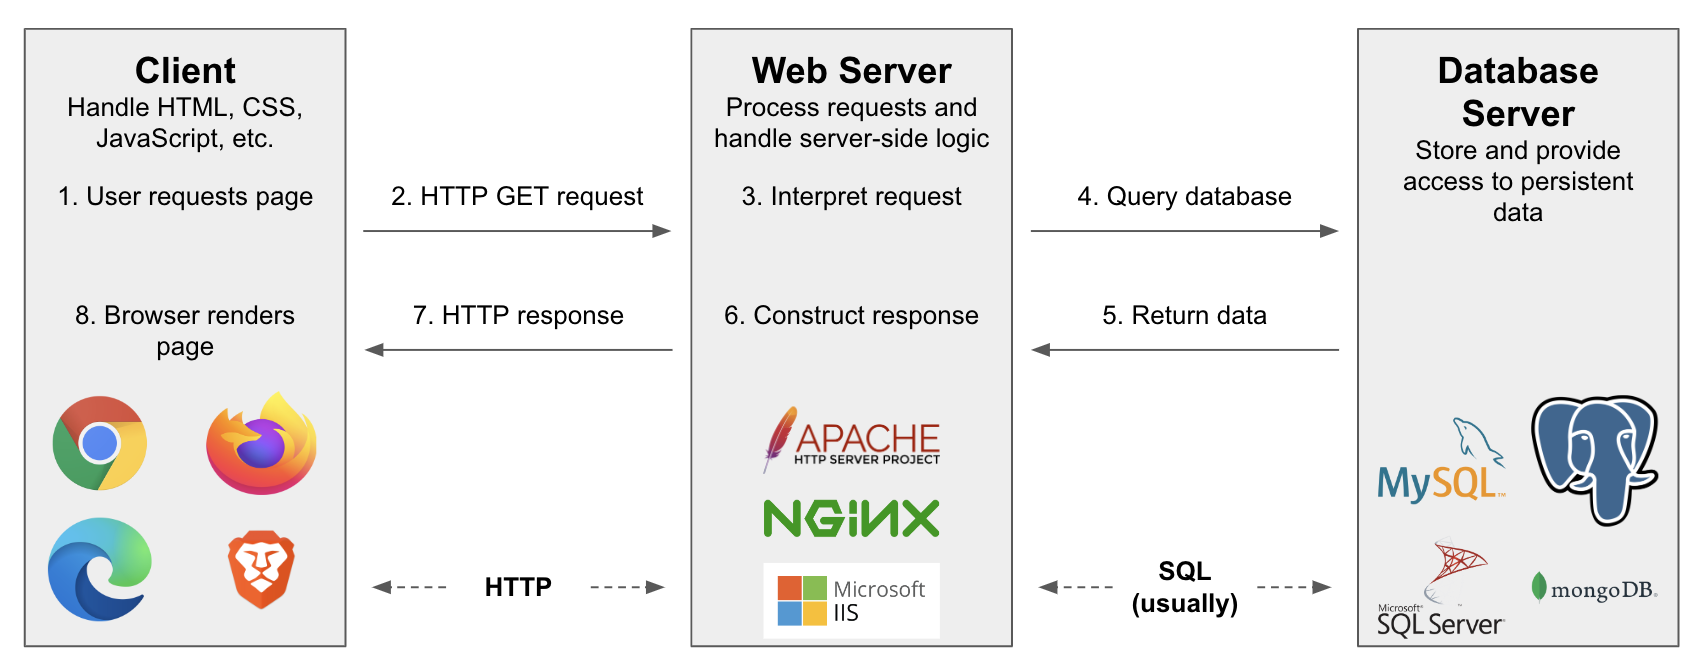
\includegraphics[width=1\linewidth]{img/lec16-img0}
  \caption{Structure of web services.}
\end{figure}

Since the web server uses user input as part of the code it runs, an attacker may \emph{inject} SQL into queries to cause malicious behavior.

\subsection{Escape inputs}
One way to defend against SQL injections is to escape any potential input that could be used in an attack. However, sanitizing the input is difficult and there are many edge cases.

\subsection{Prepared statements}
A more robust defense is prepared statements (i.e. parameterized SQL). We compile the query first and plug in user input after the query has been interpreted by the SQL parser. Since the user input is added after the query is compiled and interpreted, an attacker input is never treated as SQL code.

\subsection{Command injection}
Untrusted data can be manipulated in many languages aside from SQL. In general, the best defense is to use safe APIs.

\section{CAPTCHAs}
Robot access of websites can lead to attacks. CAPTCHAs are designed such that the problems are easy for humans but difficult for computers. The modern issue with CAPTCHAs is that as solving algorithms get better, our defense deteriorates.